\subsection{Devkit GUI - Mathias}

\subsubsection{Design}

Til den grafiske burgerflade ønskes der et meget simpelt design. Den grafiske brugerflade skal have følgende funktionaliteter:

\begin{itemize}
	\item Skal kunne starte og stoppe for udrugningssekvensenn, 
	\item Skal kunne vise den forløbne tid, samt den aktuelle temperatur og luftfugtighed.
	\item Skal give besked til brugeren, når lågen er åben.
\end{itemize}

Dette giver et basisudkast at arbejde ud fra til implementeringsfasen.

\subsubsection{Implementering}
Til at lave GUI applikationen blev der anvendt Qt frameworket. Dette blev valgt, da det er et relativt simpelt framework at benytte. Det er baseret på C++.

Idet implementeringen af GUI applikationen samtidigt var en del af læringsprocessen i Qt, blev implementeringen meget metodisk. 

For at give et godt udgangspunk at arbejde ud fra, blev den grafiske del af programmet først implementeret. Det endelige grafiske design, implementeret i Qt, kan ses på figur \ref{fig:GUI}.

\begin{figure}[H]
\centering
\fbox{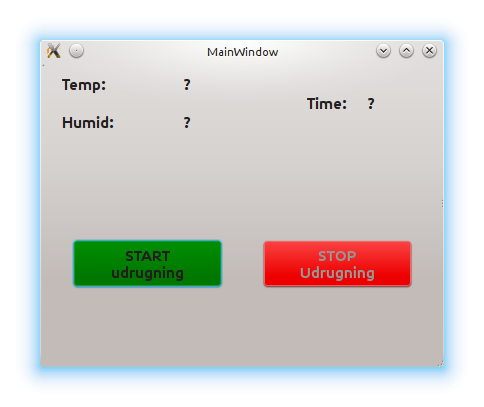
\includegraphics[page=1,width=((\linewidth)/10)*8]{./7_projektbeskrivelse/design_og_implementering/software/billeder/GUI.png}}
\caption[Figur]{GUI designet, implementeret i Qt.}
\label{fig:GUI}
\end{figure}

I designfasen blev den grafiske del holdt meget simpelt for at gøre det simpelt at implementere. Der blev derfor hurtigt lagt vægt på at få implementeret den underliggende software til applikationen.

 Der blev derfor udarbejdet et UML klassediagram for at give et overblik over de forskellige klasser, der skulle laves, deres relationer, samt nedarvningshierarki. Ligeledes blev det brugt til at give overblik over de forskellige metoder, der skulle laves under de forskellige klasser:

\begin{figure}[H]
\centering
\fbox{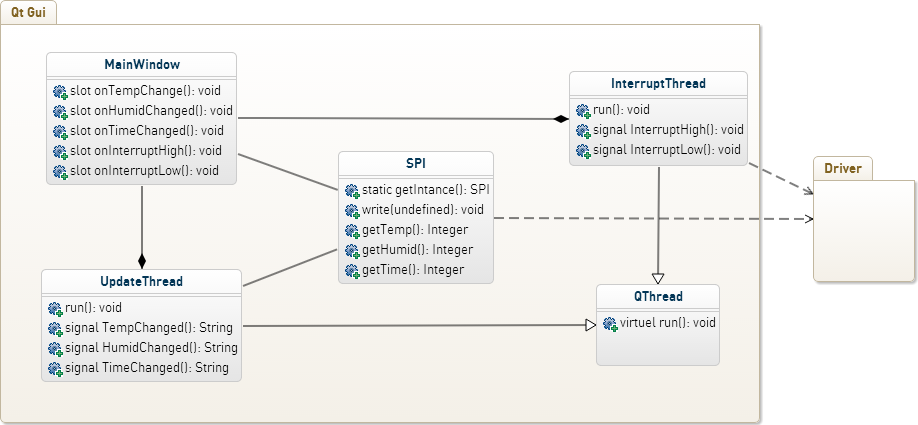
\includegraphics[page=1,width=\linewidth]{./7_projektbeskrivelse/design_og_implementering/software/billeder/klasse_diagram.png}}
\caption[Figur]{Klasse diagram over GUI applikationen.}
\label{fig:klasse_diagram}
\end{figure}

For at lave en grafisk applikation, som fungerer så flydende som muligt, blev der anvendt flertrådet programmering. Det blev valgt, at der blev benyttet en "main" tråd til at håndtere selve den grafiske, eventorienterede programmeringsdel. Der blev dertil lavet to datatråde, som hver især står for at skulle håndtere data og sende til "main" tråden. De to tråde blev lavet som klasserne UpdateThread og InterruptThread og blev, ud fra Qt dokumentationen omkring flertrådet programmering, lavet som nedarvninger fra klassen Qthread \footnote{Se Starting Threads with QThread\cite{Qthread}}.


\textbf{MainWindow:}
\texttt{MainWindow} er klassen, der står for at håndtere selve "main" vinduet. Klassen har nogle metoder, der håndterer de to trykknapper samt nogle forskellige slots. De forskellige slots anvendes til at fange signaler emittet fra de to andre tråde. 

\texttt{MainWindow} står for at oprette de to datatråde \texttt{InterruptThread} og \texttt{UpdateThread} og har kendskab til SPI klassen.

\textbf{SPI:}
SPI klassen er en klasse, der er tilpasset til at tage sig af kommunikationen til PSoC3 via den udarbejde driver. SPI klassen opretter derfor tre C++ file streams til at gå ud og læse på de tre driver nodes med temperatur, luftfugtighed og tid. Til at håndtere skrivningen over SPI kommunikationen blev der anvendt et C file handle. Dette blev anvendt frem for C++ fil behandlingen, da der er større kontrol over buffere, når der anvendes almindelig C. Da der er flere tråde, der skal kunne anvende SPI klassen, blev den givet en mutex, som den i hver af \texttt{get} og \texttt{write} metoderne låser i starten og frigives i slutningen. For at sikre at trådsynkroniseringen bliver holdt, er det nødvendigt, at der kun benyttes en fælles instans af klassen af de andre klasser. Det blev gjort via metoden \texttt{getInstance}, samt en privat constructor. SPI klassen kan derfor kun tilgås via metoden \texttt{getInstance}:

\begin{lstlisting}
SPI& SPI::getInstance()
{
    static SPI spi;
    return spi;
}
\end{lstlisting}

Idet metoden er erklæret static, kan metoden tilgås, selvom der ikke er oprette en instans af klassen. Første gang metoden så kaldes, opretter den en static instans af SPI klassen, som den så returnerer en reference dertil. Dette sikrer, at når metoden kaldes næste gang, er instansen allerede oprettet.

\textbf{UpdataThread:}
Klassen \texttt{UpdataThread} bruges til at gå ud og hente temperatur, luftfugtighed og tid, via SPI klassen. \texttt{UpdateThread} står herefter for at lave de hentede integer værdier om til Qstrings, med det ønskede formatering, og emitte de forskellige signaler til \texttt{MainWindow}, som så viser data'en.

\textbf{InterruptThread:}
\texttt{InterruptThread} står for at læse på interrupt linien i driveren. \texttt{InterruptThread} emmitter så et signal alt efter hvilken værdi der læses fra driveren. Hvis der sendes en \texttt{interruptHigh}, vises der en \texttt{Qmessagebox}, der informerer brugeren om, at lågen er åben. \texttt{InterruptLow} står så for at lukke denne \texttt{Qmessagebox} igen. 